\documentclass{article}
\usepackage{amsmath}
\usepackage{amssymb}
\usepackage{graphicx}
\usepackage{hyperref}
\usepackage[version=4]{mhchem}

\title{Example 10}
\date{}

\begin{document}
\maketitle

\(A B\) is the diameter of circle \(O\). Extend \(A B\) to \(D\) such that \(B D=O B\). \(D C\) is tangent to the circle at \(C\). Find the measure of \(\angle A\).

Solution: \(30^{\circ}\).\\
Connect \(O C, B C\).\\
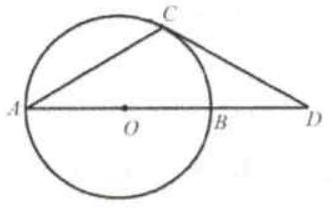
\includegraphics[width=\textwidth]{images/problem_image_1.jpg} \(\angle D C O=90^{\circ}\).\\
Since \(B D=O B, B C\) is the median of right triangle \(D C O\). Thus \(B D=O B=B C=\) CO.\\
Triangle \(B C O\)\\
is an equilateral triangle and \(\angle C O B=60^{\circ}\).\\
Since \(\angle C O B\) is the central angle and \(\angle A\) is the inscribed\\
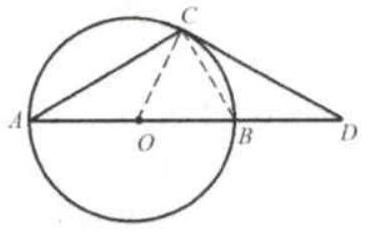
\includegraphics[width=\textwidth]{images/reasoning_image_1.jpg} angle facing the same arc \(B C, \angle A=\frac{1}{2} \angle C O B=30^{\circ}\).


\end{document}
